\begin{exsol}{16}{Tadelis Exercise 8.13}{173--174}{Exam}{L3}
\asked A buyer pays a commuting cost $k$ to reach a seller, who then names a take-it-or-leave-it
price. (a) Extensive form and the buyer's reply at the acceptance node; (b) the SPE, its
uniqueness and Pareto optimality; (c) Nash equilibria better for both; (d) whether the seller
would pay $\varepsilon$ to mail a postcard that commits him to a price.

\method Backward induction with a continuum of actions (Tadelis \S8.1 and \S8.3.2, the
Stackelberg logic, pp.~160--163); the ultimatum-game argument for ties (Tadelis Prop.~11.2,
p.~223: the responder must accept at indifference, or the proposer has no best offer). Nash
equilibria sustained by off-path threats (Tadelis Def.~7.8, p.~146). Commitment as a move added
before the game (\texttt{Notas/L03/L03-06}, Cabral \S7.2).

\solution
\textbf{Notation.} Buyer (B) and seller (S). B chooses $G$ (go to the store) or $H$ (stay
home); then S names $p \ge 0$; then B accepts ($Y$) or walks out ($N$). Data: $c > 0$,
$k > 0$, $v > c + k$. Payoffs $(u_B, u_S)$:
\[
  H:\ (0,\ c);\qquad G,p,Y:\ (v - p - k,\ p);\qquad G,p,N:\ (-k,\ c).
\]

\textbf{(a) Extensive form and the buyer's reply.}
\begin{center}
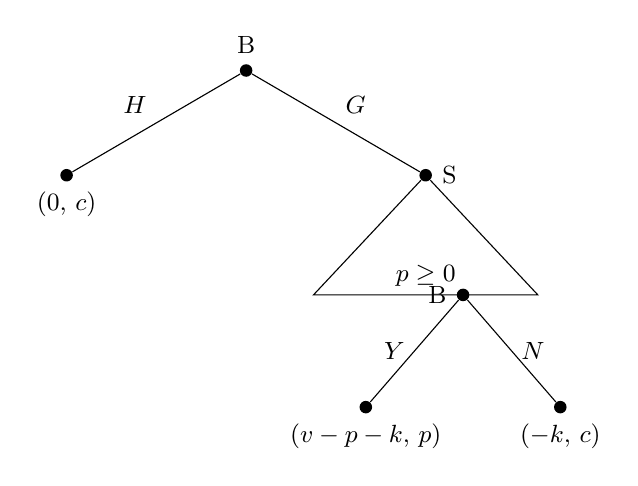
\begin{tikzpicture}[scale=0.95,dot/.style={circle,fill,inner sep=1.6pt},
  every node/.style={font=\small}]
  \node[dot,label=above:{B}] (r) at (0,0) {};
  \node[dot,label=below:{$(0,\,c)$}] (h) at (-2.4,-1.4) {};
  \node[dot,label=right:{S}] (s) at (2.4,-1.4) {};
  \draw (r) -- node[above left] {$H$} (h);
  \draw (r) -- node[above right] {$G$} (s);
  \draw (s) -- (0.9,-3.0) -- (3.9,-3.0) -- (s);
  \node at (2.4,-2.75) {$p \ge 0$};
  \node[dot,label=left:{B}] (b) at (2.9,-3.0) {};
  \node[dot,label=below:{$(v-p-k,\,p)$}] (y) at (1.6,-4.5) {};
  \node[dot,label=below:{$(-k,\,c)$}] (n) at (4.2,-4.5) {};
  \draw (b) -- node[left] {$Y$} (y);
  \draw (b) -- node[right] {$N$} (n);
\end{tikzpicture}\\[2pt]
{\footnotesize The triangle stands for the continuum of prices; one typical price $p$ is drawn.}
\end{center}
At the node after price $p$, the commuting cost is already sunk; it appears in both payoffs. B
accepts if
\[
  v - p - k \;\ge\; -k \iff p \le v .
\]
So the best reply is: accept every $p < v$, reject every $p > v$, and either action at $p = v$.

\textbf{(b) SPE, uniqueness, efficiency.}

\emph{Step 1: the acceptance rule at $p = v$.} Suppose B rejected $p = v$. Then S would get $p$
for every $p < v$ and $c < v$ otherwise, so his payoff approaches $v$ as $p \uparrow v$ but never
reaches it; S would have no best offer, so the profile cannot be an SPE. Hence in every SPE B
accepts if and only if $p \le v$.

\emph{Step 2: the seller.} Given that rule, S's payoff is $p$ for $p \le v$ and $c < v$ for
$p > v$; the unique maximizer is $p^* = v$.

\emph{Step 3: the buyer's commuting decision.} Going yields
\[
  u_B(G) = v - p^* - k = v - (v) - k = -k \;<\; 0 = u_B(H),
\]
so B stays home. Every step had a unique optimum, so the SPE is unique:
\[
  \text{B: } H\text{, and accept iff } p \le v;\qquad \text{S: offer } p = v. \qquad
  \text{Outcome: no trade, payoffs } (0,\ c).
\]
\emph{Not Pareto optimal.} Trade at any price $p \in (c,\ v - k)$ (nonempty since $v > c+k$)
gives $u_B = v - p - k > 0$ and $u_S = p > c$: both strictly better. The lost surplus is
$v - c - k > 0$. This is a hold-up: the commuting cost is sunk when the price is set, so S
extracts all of $v$ and B, anticipating it, never makes the trip.

\textbf{(c) Better Nash equilibria.} Yes. Fix $\hat p \in (c,\ v - k)$ and consider
\[
  \text{B: } G\text{, accept iff } p \le \hat p;\qquad \text{S: offer } \hat p .
\]
\emph{S's best reply:} offers $p \le \hat p$ are accepted and give $p \le \hat p$; offers above are
rejected and give $c < \hat p$. So $\hat p$ is optimal. \emph{B's best reply:} given $\hat p$,
going and accepting gives $v - \hat p - k > 0$, more than staying (0) or going and rejecting
($-k$); B's rule at prices other than $\hat p$ is off the path and does not affect his payoff.
Payoffs $(v - \hat p - k,\ \hat p)$ beat $(0, c)$ for both. It is not subgame perfect: after an
off-path offer $p \in (\hat p, v)$, rejecting gives $-k < v - p - k$, so the threat to walk out
is not credible.

\textbf{(d) The postcard.} Add a first move: S either mails a postcard committing to $\hat p$ (at
cost $\varepsilon$) or does not. Without the postcard the game is the one in (b): payoff $c$ to S.
With it, B buys at $\hat p$ if he goes and $\hat p \le v$, so he goes iff
$v - \hat p - k \ge 0$, i.e.\ $\hat p \le v - k$. By the argument of Step~1, B goes at
indifference. Then S's payoff from the postcard is
\[
  u_S(\hat p) = \begin{cases} \hat p - \varepsilon, & \hat p \le v - k,\\
  c - \varepsilon, & \hat p > v - k, \end{cases}
  \qquad\Rightarrow\qquad \hat p^* = v - k,\quad u_S = v - k - \varepsilon .
\]
Compared with not mailing,
\[
  (v - k - \varepsilon) - c = (v - c - k) - \varepsilon > 0
  \quad\text{since } \varepsilon < v - c - k .
\]
So in the SPE the seller mails the postcard with price $v - k$; B goes and buys; payoffs
$(0,\ v - k - \varepsilon)$. Trade now happens; the total surplus is $v - c - k - \varepsilon$, all
of it to the seller.

\interp The commitment in (c) has to come from the buyer and is not credible; the commitment in
(d) comes from the seller, who limits his own future options, and it is credible because the
coupon binds him. ``Junk mail'' has value even when it contains no information: it is a
commitment not to hold up a customer who has sunk a cost. The seller still captures the whole
surplus; the coupon only removes the inefficiency, the same logic as the bond in the entry game
(Cabral \S7.2).

\verify \texttt{check\_B\_L03.py} uses $c = 2$, $v = 10$, $k = 1$, $\varepsilon = \frac12$ and prices
on a $0.25$ grid: the seller's best offer is $p = 10 = v$ and the buyer stays home; under
``reject at $v$'' the best grid offer is $v - 0.25$ (no maximum on a continuum); thresholds
$\hat p \in \{2.5, 5, 8.5\}$ give Nash equilibria that beat $(0, c)$ for both; with the postcard,
$\hat p^* = 9 = v - k$ and $8.5 > 2$; sympy confirms the gain $(v - c - k) - \varepsilon$. Tadelis
prints no answer.

\answer{(a) Tree above; at the acceptance node the buyer accepts iff $p \le v$ (the sunk $k$ does
not matter). (b) Unique SPE: seller offers $p = v$, buyer accepts iff $p \le v$ and therefore stays
home; payoffs $(0, c)$; not Pareto optimal, since trade at any $p \in (c, v-k)$ helps both. (c) Yes:
buyer goes and accepts only $p \le \hat p$, seller offers $\hat p$, for any $\hat p \in (c, v-k)$;
Nash but not subgame perfect. (d) Yes: the seller mails a coupon at $\hat p = v - k$, the buyer
comes and buys, seller earns $v - k - \varepsilon > c$.}
\end{exsol}
